\documentclass[sigconf]{acmart}


\usepackage{tikz}
\usepackage{pgfplots}
\usepackage{pgfplotstable}
\usepackage{subcaption}
\usepackage{multirow}
\usepackage{multicol}
\usepackage[table]{xcolor}
\usepackage{colortbl}
\usepackage{graphicx}
\usepackage{array}
\usepackage{float}
\usepackage{blindtext}
\usepackage{enumitem}
\usepackage{tcolorbox}
\usepackage{verbatim}
\usepackage{quoting}


\pgfplotsset{compat=1.18}
\usetikzlibrary{patterns}

\definecolor{good}{rgb}{0.267004, 0.004874, 0.329415}   % Dark purple
\definecolor{okay}{rgb}{0.190631, 0.407061, 0.556089}   % Blue-green
\definecolor{notgood}{rgb}{0.368627, 0.788888, 0.482758} % Yellow-green
\definecolor{bad}{rgb}{0.993248, 0.906157, 0.143936}    % Yellow

\AtBeginDocument{%
  \providecommand\BibTeX{{%
    \normalfont B\kern-0.5em{\scshape i\kern-0.25em b}\kern-0.8em\TeX}}}

\copyrightyear{2024}
\acmYear{2024}
\setcopyright{rightsretained}
\acmConference[ITiCSE 2024]{Proceedings of the 2024 Conference on Innovation and Technology in Computer Science Education V. 1}{July 8--10, 2024}{Milan, Italy}
\acmBooktitle{Proceedings of the 2024 Conference on Innovation and Technology in Computer Science Education V. 1 (ITiCSE 2024), July 8--10, 2024, Milan, Italy}\acmDOI{10.1145/XXXXXX.XXXXXX}
\acmISBN{979-8-4007-XXXX-X/XX/XX}

\begin{document}

\title[]{}


%%
%% The "author" command and its associated commands are used to define
%% the authors and their affiliations.
%% Of note is the shared affiliation of the first two authors, and the
%% "authornote" and "authornotemark" commands
%% used to denote shared contribution to the research.

\author{Anon Author}
\orcid{}
\affiliation{
  \institution{University of Anon}
  \city{Anonville}
  \country{Rep. of Anon}
}
\email{anon@anonuni.edu}

\author{Anon Author}
\orcid{}
\affiliation{
  \institution{University of Anon}
  \city{Anonville}
  \country{Rep. of Anon}
}
\email{anon@anonuni.edu}

\author{Anon Author}
\orcid{}
\affiliation{
  \institution{University of Anon}
  \city{Anonville}
  \country{Rep. of Anon}
}
\email{anon@anonuni.edu}

\author{Anon Author}
\orcid{}
\affiliation{
  \institution{University of Anon}
  \city{Anonville}
  \country{Rep. of Anon}
}
\email{anon@anonuni.edu}


%\renewcommand{\shortauthors}{Anon Author, et al.}

\renewcommand{\shortauthors}{}



\begin{abstract}

    \textbf{Background:} 

    \noindent\textbf{Objective:} 

    \noindent\textbf{Method:} 

    \noindent\textbf{Results:} 
\end{abstract}


%%
%% The code below is generated by the tool at http://dl.acm.org/ccs.cfm.
%% Please copy and paste the code instead of the example below.
%%
\begin{CCSXML}
<ccs2012>
  <concept>
   <concept_id>10003456.10003457.10003527</concept_id>
   <concept_desc>Social and professional topics~Computing education</concept_desc>
   <concept_significance>500</concept_significance>
   </concept>
  <concept>
   <concept_id>10010147.10010178</concept_id>
   <concept_desc>Computing methodologies~Artificial intelligence</concept_desc>
   <concept_significance>500</concept_significance>
   </concept>
 </ccs2012>
\end{CCSXML}

\ccsdesc[500]{Social and professional topics~Computing education}
\ccsdesc[500]{Computing methodologies~Artificial intelligence}

%%
%% Keywords. The author(s) should pick words that accurately describe
%% the work being presented. Separate the keywords with commas.
\keywords{}

\maketitle

\section{Introduction}





In \citet{jordan2024need}, they found that amoung the languages under their
consideration, English, Spanish, Vietnamese, and Tamil, the worst performing
language was Tamil, generating incorrect solutions and non-sensiable
translations. Though the authors did not systematically investigate the the
nature of the poor performance or methods of improvement, they did note several
possible reasons:
\begin{enumerate}
  \item 
  \item Compared to English and Spanish it was likely a lower resourced language
    in the training data.
\end{enumerate}
The first of these two possibilities is, perhaps, the most interesting. In
Tamil, there are two core dialects which differ significantly: literary Tamil
(sen-Tamil) and colloquial (kodun-Tamil)~\cite{}. Additionally, given Tamil is
spoken not just in and around Tamil Nadu, but also in Sri Lanka, Malaysia, and
Singapore, there are a number of regional dialects~\cite{}. 


\section{Background}


\begin{table*}[ht]
\centering
\renewcommand{\arraystretch}{1.8}
\begin{tabularx}{\textwidth}{>{\bfseries\raggedright\arraybackslash}X >{\raggedright\arraybackslash}X >{\raggedright\arraybackslash}X >{\raggedright\arraybackslash}X} 
  \hline
\rowcolor{steelblue}
\textcolor{white}{NEP Edition} & \textcolor{white}{\textbf{1968}~\cite{NEP1968}} &
\textcolor{white}{\textbf{1986}~\cite{NEP1986}} &
\textcolor{white}{\textbf{2020}~\cite{NEP2020}} \\ \hline
\rowcolor{palesteelblue}
Hindi-Speaking States & Hindi, English, and a modern Indian language (preferably from Southern India) & Hindi, English, and a modern Indian language (preferably from Southern India) & Three languages of the student's or state's choice (at least two must be native to India) \\
\rowcolor{white}
Non-Hindi Speaking States & Regional language, Hindi, and English & Regional language, Hindi, and English & Three languages of the student's or state's choice (at least two must be native to India) \\
\rowcolor{palesteelblue}
Key Change & First formal introduction of the formula to promote national
integration & Reiterated the 1968 formula without changes & Introduced
flexibility, allowing students to choose the languages, with the condition that
two of the three languages must be Indian \\ \hline
\end{tabularx}
\vspace{0.5em}
\caption{Evolution of the Three-Language Formula in National Education Policies}
\label{tab:three-language-formula}
\end{table*}

To situate the work presented in this paper, we provide an overview of four
relevant sources of literature. First, in
Section~\ref{subsec:indian-higher-education}, we provide a broad overview of the
Indian higher education system with a particular focus on the role that
multilingualism plays in shaping policy and practice. Next, in
Section~\ref{subsec:theories-of-translanguaging},

\subsection{Indian Higher Education \& Language}~\label{subsec:indian-higher-education}

Here, we provide a broad overview of Indian higher education both from the
perspectives of policy and practice. In
Sections~\ref{subsubsec:multilingualism-in-indian-education} and
\ref{subsubsec:language-and-education-policy}, we discuss the multilingual
nature of India and Indian education, respectively. We follow this with an
overview of emperical work on language and Indian higher education in
Section~\ref{subsubsec:emperical-work}.

\subsubsection{Multilingual Landscape}\label{subsubsec:multilingualism-in-indian-education}

% Indian lnguistic landscape
The linguistic landscape of India is incredibly diverse, to such an extent that
it can be difficult to exaclty quantify the number of languages spoken in the
country. India has 22 scheduled languages---meaning they are officially
recognized by the government and have a special status in the constitution---and 
many hundreds of other languages and dialects that are spkoken arcoss its 28
states and 8 union territories~\cite{2011census}.


\subsubsection{Language and Education
Policy}\label{subsubsec:language-and-education-policy}

% NEP and the three language policty
India's National Education Policy (NEP) of 2020~\cite{NEP2020} emphasizes the importance of
of equity and the centrality of language in achieving equitable education.
\begin{quote}
  ``\textit{The aim must be for India to have an education system by 2040 that
  is second to none, with equitable access ot the highest quality educaiton for
  all learners regardless of social or ecenomic background}''(p. 3)
\end{quote}
In previous editions of the NEP, which took places in 1968 and 1980, the
three-language formula has been a key policy in Indian education system---though
it has undergone considerable evolution in it's most recent iteration
(Table~\cite{tab:three-language-formula }). This policy mandates that students
learn three languages where the specific languages differed based primarily on
whether a student lived in a Hindi or non-Hindi speaking state. The 2020 edition
of the NEP, though continuin to emphasize the importance of learning three
languages introuces greater flexibility in which languages fit into each
category and leaves it to the state or region to make these policy decision.

\subsubsection{Emperical Work}\label{subsubsec:emperical-work}


\subsection{Language and Computing Education}

% The rise of natural language programming
Programming, once the domain of structured syntax and rigid semantics, is
increasingly shifting towards natural language interfaces for program
specification~\cite{lau2023ban, prather2025beyond, chen2025empirical,
petrovska2024incorporating}---courtesy of the advanced program synthesis
capabilities of large language models~\cite{austin2021program, jimenezswe}. The
prevelance of English venacular in programming language keywords and
documentation has long been a barrier to entry for non-English
speakers~\cite{guo2018non}. However, the shift towards natural language
prompts---brought about courtesy of multilingual GenAI models, presents both
new opportunities as well as new challenges for non-English speakers. Below, we
highlight some of the key challenges non-English speaking novice programers
have faced historically as well as some of the opprotunities that may arise as
programming moves towards natural language interfaces.

\subsubsection{Potential Challenges for non-English Speakers}



% Role of Syntax and Language
As noted, by \citet{guo2018non}, the vast majority of programming
languages---and almost centainly all widely adopted programming
languages---rely on English keywords. \citet{stefik2013emperical} compared
error rates by novice programmers among a variety of programming languages
(i.e., Quorum, Python, Java, C, Pearl) to that of a language that used random
keywords (i.e., Randomo). They found that languages that used syntax that more
naturally resembled natural language (i.e., Quorum and Python) had lower error
rates and that students had similar error rates for Randomo and languages like
Java. This not only highlights the role that syntax plays but, as hypothesized
by \citet{becker2019parlez}, that non-English speakers may not be able
to share in the affordances of languages such as Quorum and Python. This
hypothesis was, in part, confirmed by the work of \citet{dasgupta2017learning}
which found that Scratch users coding in their localized native language
demonstrate new programming concepts at a faster rate than users from the same
countries using English interfaces, controlling for activity levels and
socialization. 


As noted---somewhat profetically in retreospect given it was published before
widely availbe GenAI models---by \citet{becker2019parlez} as programming
language design moves away from random keywords, to keywords that invoke
natural language, towards fully natural language interface, the difficulty gap
in aquiring that language will become steadily larger and favor the user who is
already familiar with the natural language which the interface is based on. 
\begin{quote}
   ''However, imagine if perfect natural (English) language programming was
   achievable today.''
\end{quote}
Imagine indeed. However, we are fortunate in that large language models are
trained on a wide variety of languages, suggesting that interfacing with these
models in non-English languages may be possible and thus lower the barrier to 
entry for non-English speakers.


\subsubsection{Opportunities for non-English Speakers}

Perhaps the immediate, and most obvious, opportunity is the ability to interact
with programming environments in one's native language~\cite{smith2024explain,
li2024bridging, raihan2024mhumaneval, prather2025breaking}.
As noted by 



\subsubsection{India Specific Opportunities and Challenges}

\citet{bhattacharyya2019indic} characterized a wide variety of challenges relating
to Indic languages and computing. These included, 
\begin{enumerate} 
  \item \textbf{Scale and Diversity}
  Indic languages encompass a vast array of languages and dialects, belonging to multiple linguistic families and written in numerous distinct scripts.
  \item \textbf{Longer Utterances}
    Sentences in Indic languages are often longer and more complex than in English, complicating tasks like parsing and speech recognition.
  \item \textbf{Code Mixing}
    The frequent mixing of multiple languages in a single sentence or conversation is a common challenge in computational linguistics for the region.
  \item \textbf{Resource Scarcity}
    Many Indic languages lack sufficient annotated datasets for building robust NLP and speech tools.
  %\item \textbf{Absence of basic speech and NLP tools}
  %  Foundational tools like morphology analyzers and speech recognition systems are either unavailable or lack accuracy for most Indic languages.
  \item \textbf{Absence of linguistics knowledge}
    A limited understanding of the linguistic structure of many regional languages hinders the development of computational models.
  \item \textbf{Script complexity and non-standard input mechanisms}
    The diversity of scripts and their associated vowel and consonant combinations make input systems slower and less intuitive.
  \item \textbf{Non-standard transliteration}
    Roman transliteration of Indic languages lacks standardization, leading to multiple ways of representing the same word.
  %\item \textbf{Non-standard storage}
  %  Variations in how characters are encoded and stored pose issues in data sharing and tool interoperability.
  %\item \textbf{Man-made Problems}
  %  Government-imposed standard keyboards and inadequate funding often stifle innovation and efficiency in linguistic computing.
  %\item \textbf{Some challenging language phenomena}
  %  Features like free word order, agglutination, and context-dependent pronunciation introduce additional computational hurdles.
\end{enumerate}
Though issues such as \textit{}

\citet{} found that 
\citet{smith2024explain} had similar findings with Tamil translations of
correct English descriptions of code having far less success than 10 other of
hte most commonly spoken languages in India



\subsection{Pedagogy and Linguistic Diversity}

\subsubsection{Theories of Translanguaging}

% Definitions, terms, etc

% Theories of translanguaging

% Translanguaging work in india






\section{Methods}

We developed a semi-structured interview protocol to explore how educators
across a variety of tertiary insitutions. In
Section~\ref{subsec:interview-questions}, we describe the interview questions
that we developed and in Subsection~\ref{subsec:interview-probes} we describe
the taxonomy of interview probes we empoloyed to guide consistent follow-up
questions across interviews. Following this, in
Section~\ref{sec:data-collection} we describe our recruitment and data
collection procedures. Finally, in Section~\ref{sec:data-analysis} we describe
our approach to analyzing the data collected through these interviews.

\begin{figure*}[ht]
  \centering
  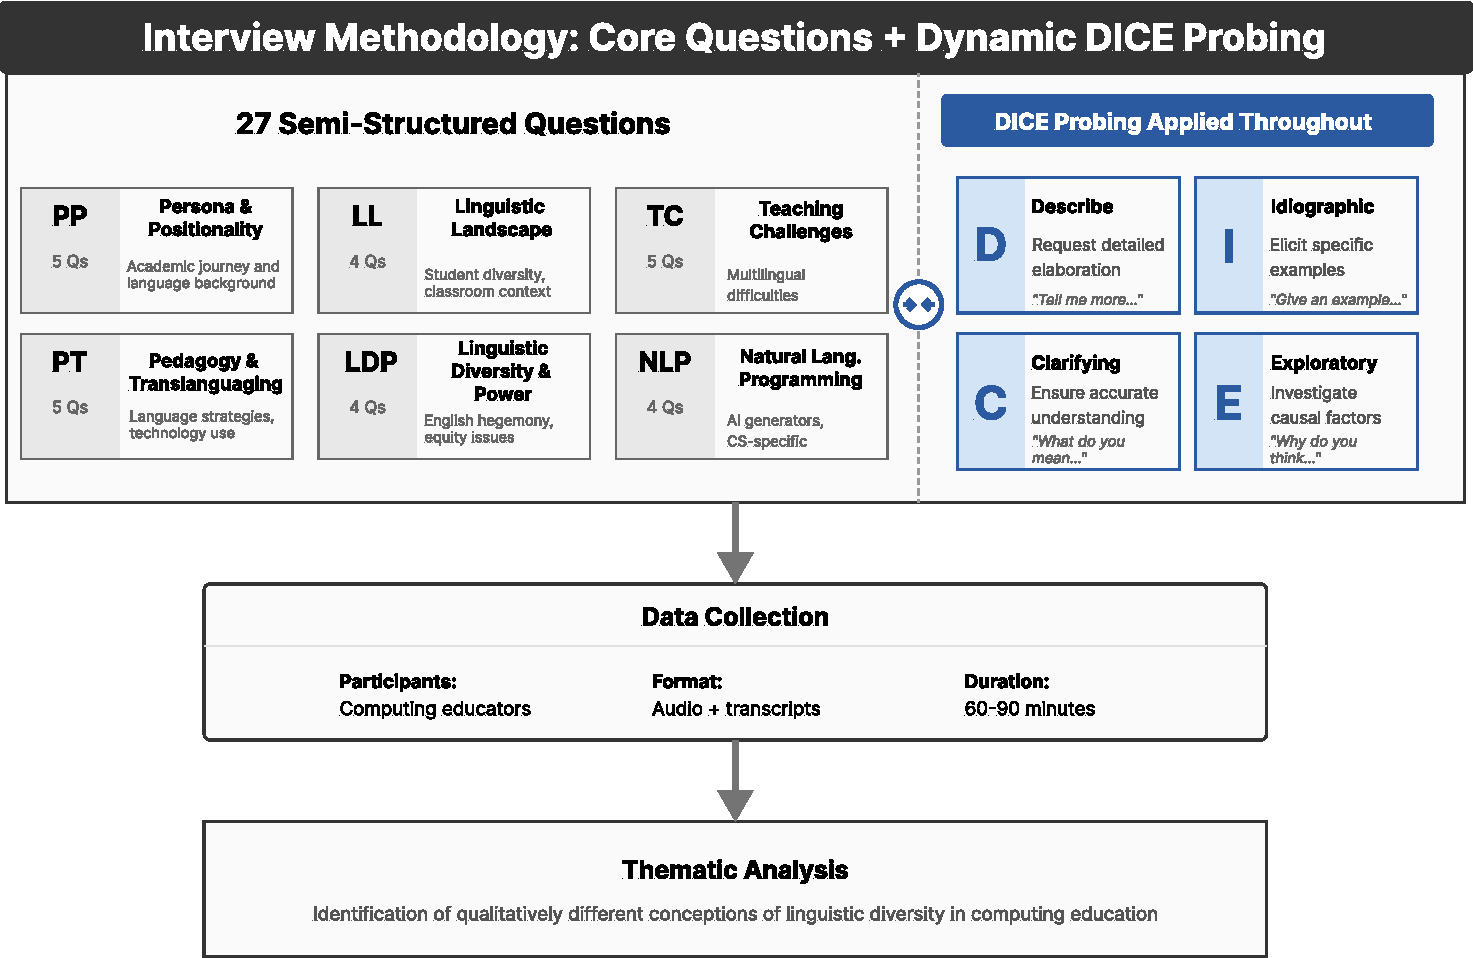
\includegraphics[width=\textwidth]{imgs/methods.pdf}
  \caption{Your caption here.}
  \label{fig:methods}
\end{figure*}


\subsection{Interview Questions}\label{subsec:interview-questionse

\subsubsection{Persona and Positionality}\label{subsubsec:persona-and-positionality}

% Context and grounding
Given the phenomenographic nature of this work, it is important that we
understand the context and positionality of each participant. These questions
are designed to provide this context---with particular focus on the
educational, instructional, and linguistic backgrounds of each participant. The
questions, in this regard, are as follows:
\begin{enumerate}[label={PP.\arabic*}, align=left, leftmargin=4em]
  \item Could you briefly describe your academic journey and how you came to
    teach in your current position?
  \item What subjects do you currently teach, what levels (e.g., undergraduate,
    graduate) are these courses, and in what contexts (e.g., in-person, online,
    hybrid) are they delivered?
  \item What languages do you speak, and in what contexts do you typically use
    each?
  \item In your own education, what language(s) were used for instruction?
  \item What are your general thoughts and beliefs about the role of language in
    education, particularly in technical fields like computer science?
\end{enumerate}
Probes during this section of the interview focused on understanding
\textcolor{red}{TBD}.

\subsubsection{Linguistic Landscape}\label{subsubsec:linguistic-landscape}

Related to understanding the persona of each participant, it is essential to
underastand the linguistic landscape in which they operate. This includes not
only the languages spoken by their students, but also the languages used in
instruction
\begin{enumerate}[label={LL.\arabic*}, align=left, leftmargin=4em]
  \item How would you describe the linguistic diversity of your current students? 
  \item Your second question here
\end{enumerate}

\subsubsection{Teaching Challenges}\label{subsubsec:teaching-challenges}

\begin{enumerate}[label={TC.\arabic*}, align=left, leftmargin=4em]
  \item What are the biggest challenges you face teaching topics in
    computing to students who speak a variety of languages?
  \item Can you describe 
\end{enumerate}

\subsubsection{Pedagogy and Translanguaging}\label{subsubsec:pedagogy-and-translanguaging}

In this section, we explore the intersection of translanguaging practices and
pedagogical strategies employed by educators in multilingual settings.
\textcolor{red}{<Resaerch on india specifically and findings that inform these
questions>}.The questions are designed to uncover how educators navigate---or
leverage---the linguistic diversity of their classrooms.
\begin{enumerate}[label={PT.\arabic*}, align=left, leftmargin=4em]
  \item How do you decide when to use a particular language for
    instruction or explanation during your classes and when, if at all, do
    to change languages?
  \item If you've adopted a teaching strategy that helps you navigate
    linguistic diversity, can you describe it and why you find it effective?
  \item How do you use technology, if at all, to support students with
    different language backgrounds?
\end{enumerate}

\subsubsection{Linguistic Diversity and Power}\label{subsubsec:linguistic-diversity-and-power}

Central to language is the notion of power. The use of language carries with it
implications of power, privilege, and access. As noted by \citet{jhingran2009hundreds},
\begin{quote}
  ``\textit{English is seen as the language of power and the vehicle for getting better jobs. Even poor families in urban areas aspire to send their children to these private English-medium schools.}''
\end{quote}
Similarly, as noted by \citet{mohanty2017language}, beyond the 22 scheduled
languages, there are little instruction at the primary and secondary levels of
education which creates a systemic hierarchy of language: English and Hindi at
the top, regional scheduled languages in the middle, and minority and tribal
languages at the bottom. In this section, we explore how educators in computing
education perceptions and experiences with the role of power and privilege in
the context of linguistic diversity. 
\begin{enumerate}[label={LDP.\arabic*}, align=left, leftmargin=4em]
  \item How do you perceive the role of English in your institution and
    field of study?
  \item Have you observed any instances where language has influenced
    students' academic performance or participation in class? Can you describe
    one such instance?
  \item How do you address issues of linguistic equity in your classroom?
  \item What are your thoughts on the use of local languages versus
    English in higher education, particularly in technical fields like computer
    science?
\end{enumerate}

\subsubsection{Natural Language Programming}\label{subsubsec:natural-language-programming}

This section explores the perceptions and experiences of educators regarding
the use of natural language programming tools, such as AI-driven code
generators, in multilingual educational settings. The questions aim to uncover
how these tools are integrated into teaching practices and their impact on
students with diverse linguistic backgrounds.
\begin{enumerate}[label={NLP.\arabic*}, align=left, leftmargin=4em]
  \item What concerns or difficulties have you encountered with respect
    to linguistic diversity that you feel are specific to teaching topics in computing?
  \item Have you integrated or do you have plans to integrate any
    natural language programming tools (e.g., AI code generators) into your
    teaching? 
\end{enumerate}


\subsection{Interview Probes}\label{subsec:interview-probes}
In conducting these interviews we use probes aligned with the DICE
(\textit{``Describe, Idiographic, Clarifying, Exploratory''}) taxonomy as
described in \citet{robinson2023probing}. In more detail, the four types of
probes are:
\begin{enumerate}
  \item \textbf{Describe Probe:} These probes ask that participants provide more
    detail about a specific situation or experience they mentioned. These probes
    often take the form of \textit{``Tell me more about...''} or \textit{``Do
    you recall what was happening when...''}.
  \item \textbf{Idiographic Probe:} These probes encourage participants to share
    a specific example from a specific period of time. These probes often take
    the form of \textit{``Can you give me an example of...''} or \textit{``Do
    you recall what was happening the week you...''}.
  \item \textbf{Clarifying Probe:} These probes are used to ensure that the interviewer
    accurately understands what the participant is saying. These probes often
    take the form of \textit{``What do you mean by...''} or \textit{``Can you
    expand on...''}.
  \item \textbf{Exploratory Probe:} These probes encourage participants to think
    about the causal factors or underlying reasons behind their thoughts,
    opinions and experiences. Such questions take the form of \textit{``Why do
    you that happened?''} or \textit{``What do you think led to...''}.
\end{enumerate}
This taxonomy is designed to help interviewers structure follow-up questions in
a way that encourages participants to provide rich, detailed responses. 



\subsection{Data Collection}\label{sec:data-collection}



\subsection{Data Analysis}\label{sec:data-analysis}


\section{Results}

\input{sections/03-results}

\section{Discussion}

\input{sections/04-discussion}

\section{Limitations}

\input{sections/05-limitations}

\section{Conclusion}

\input{sections/06-conclusion}


\bibliographystyle{ACM-Reference-Format}
\balance
\bibliography{refs}


\end{document}
